% Figure: Bayes conditioning.  The prior is a density over OBJECT space; the
% likelihood is a WEIGHT FIELD over that same object space; the posterior is the
% prior reweighted.  Two routes reach the same conditional.  Design width ~168mm.
\documentclass[border=0pt]{standalone}
\usepackage{amsmath,amssymb}
% Shared visual language for the figures of the book.
% Every figure in this directory loads this file so the chapter reads as one system.
% NOTE: no blank lines are allowed inside \tikzset{...} (a blank line emits \par
% and breaks key scanning).
\NeedsTeXFormat{LaTeX2e}
\ProvidesPackage{figstyle}[2026/10/21 Figure style for Free Energy to LLMs]

\RequirePackage{tikz}
\usetikzlibrary{arrows.meta,positioning,calc,fit,shapes.geometric,shapes.misc,%
  backgrounds,matrix,decorations.pathreplacing,decorations.markings,patterns.meta}

% ---------------------------------------------------------------- palette
% Same values as book/preamble/style.tex, prefixed with F.
\definecolor{FNavy}{HTML}{14324A}
\definecolor{FTeal}{HTML}{0E7490}
\definecolor{FSky}{HTML}{E7F5F8}
\definecolor{FOrange}{HTML}{D97706}
\definecolor{FAmber}{HTML}{FFF3D6}
\definecolor{FInk}{HTML}{1F2937}
\definecolor{FSlate}{HTML}{64748B}
\definecolor{FMist}{HTML}{F5F7FA}
\definecolor{FRose}{HTML}{9F1239}
\definecolor{FRoseMist}{HTML}{FFF1F2}

% ---------------------------------------------------------------- semantics
% Teal   = probability / model / data object
% Orange = training objective, cost, or the quantity moved through the system
% Navy   = neutral structure
% Slate  = secondary label or metadata
% Rose   = failure mode, hazard, masked-out region
\tikzset{
  % Lay figures out in millimetres.  A figure designed 168mm wide is included at
  % \textwidth, so its fonts appear at exactly the size written here.
  every picture/.style={x=1mm,y=1mm,font=\small,line cap=round,line join=round},
  % ---- block styles
  nbase/.style={draw,rounded corners=1.2pt,align=center,inner sep=2.4pt,%
    minimum height=7mm,text=FInk},
  nteal/.style={nbase,draw=FTeal,fill=FSky},
  norange/.style={nbase,draw=FOrange,fill=FAmber},
  nnavy/.style={nbase,draw=FNavy,fill=white},
  nsoft/.style={nbase,draw=FSlate!55,fill=FMist},
  nrose/.style={nbase,draw=FRose,fill=FRoseMist},
  ghost/.style={draw=none,fill=none,align=center,inner sep=1pt},
  plain/.style={draw=none,fill=none,align=center,inner sep=0pt},
  % ---- arrows
  ar/.style={-{Latex[length=1.7mm,width=1.35mm]},draw=FSlate,line width=0.75pt},
  ard/.style={ar,dashed},
  arteal/.style={ar,draw=FTeal},
  arorange/.style={ar,draw=FOrange},
  arrose/.style={ar,draw=FRose},
  thickar/.style={ar,line width=1.2pt},
  % ---- text roles
  ftitle/.style={font=\large\bfseries,text=FNavy,align=center},
  ptitle/.style={font=\small\bfseries,text=FNavy,align=center},
  ptitleo/.style={font=\small\bfseries,text=FOrange,align=center},
  lbl/.style={font=\scriptsize,text=FSlate,align=center,inner sep=1pt},
  lblt/.style={lbl,text=FTeal},
  lblo/.style={lbl,text=FOrange},
  lbln/.style={lbl,text=FNavy},
  lblr/.style={lbl,text=FRose},
  sub/.style={font=\scriptsize,text=FSlate!90,align=center,inner sep=1pt},
  monob/.style={font=\ttfamily\scriptsize,text=FInk,inner sep=1pt},
  mathb/.style={font=\small,text=FInk,inner sep=1pt},
  eqn/.style={font=\scriptsize,inner sep=1.5pt,text=FInk},
  % ---- decorations
  brace/.style={decorate,decoration={brace,amplitude=2.4pt},draw=FSlate,%
    line width=0.6pt},
  bracet/.style={brace,draw=FTeal},
  braceo/.style={brace,draw=FOrange},
  axis/.style={draw=FSlate!55,line width=0.6pt},
  guide/.style={draw=FSlate!45,line width=0.5pt,dashed},
  halolabel/.style={font=\scriptsize,text=FInk,fill=white,fill opacity=0.85,%
    text opacity=1,inner sep=1.4pt,align=center},
}

% Figure title above the drawing, anchored at the figure's top-left.
\newcommand{\figtitle}[2][0]{%
  \node[ftitle,anchor=north west,outer sep=0pt] at (#1,0) {#2};}

% Rounded panel behind a subgroup of nodes.
\newcommand{\figpanel}[3][]{%
  \node[draw=FSlate!35,fill=#3,rounded corners=2pt,inner sep=2.6mm,#1] {#2};}

\endinput

\begin{document}
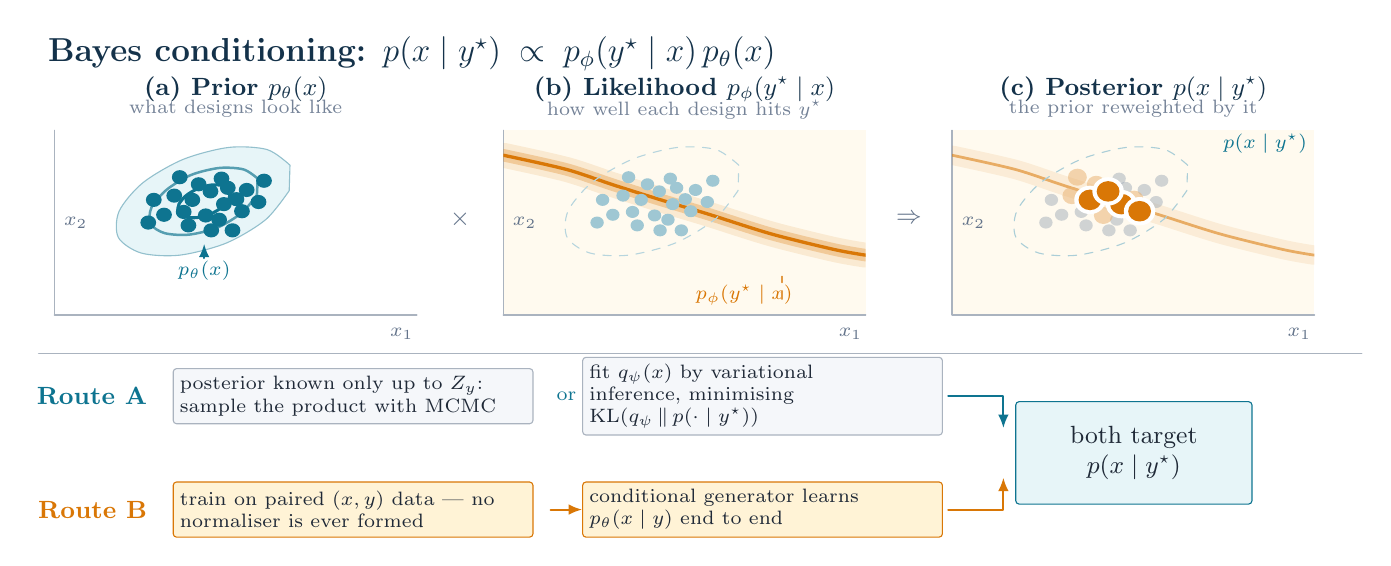
\begin{tikzpicture}[y=0.90mm]
\figtitle{Bayes conditioning: $p(x\mid y^\star)\;\propto\;p_\phi(y^\star\mid x)\,p_\theta(x)$}
% ------------------------------------------------------------------ panel titles
\node[ptitle,anchor=north] at (25,-5.5) {(a) Prior $p_\theta(x)$};
\node[sub,anchor=north] at (25,-9.8) {what designs look like};
\node[ptitle,anchor=north] at (82,-5.5) {(b) Likelihood $p_\phi(y^\star\mid x)$};
\node[sub,anchor=north] at (82,-9.8) {how well each design hits $y^\star$};
\node[ptitle,anchor=north] at (139,-5.5) {(c) Posterior $p(x\mid y^\star)$};
\node[sub,anchor=north] at (139,-9.8) {the prior reweighted by it};
% ------------------------------------------------------------------ (a) prior
\begin{scope}[shift={(2,-40.5)}]
\draw[axis] (0,0)--(46,0);
\draw[axis] (0,0)--(0,26);
\node[lbl,anchor=west] at (0.8,13) {$x_2$};
\node[lbl,anchor=north east] at (46,-1.4) {$x_1$};
\draw[draw=FTeal!45,fill=FSky,smooth] plot coordinates
  {(29.9,21.1)(27.0,23.3)(22.1,23.6)(16.3,21.9)(11.2,18.6)(8.2,14.6)%
   (8.1,10.9)(11.0,8.7)(15.9,8.4)(21.8,10.1)(26.8,13.4)(29.8,17.5)} -- cycle;
\draw[draw=FTeal!70,line width=0.9pt,smooth] plot coordinates
  {(25.8,19.2)(24.0,20.5)(20.9,20.7)(17.3,19.7)(14.2,17.6)(12.3,15.1)%
   (12.2,12.8)(14.0,11.5)(17.1,11.3)(20.7,12.3)(23.8,14.4)(25.7,16.9)} -- cycle;
\draw[draw=FTeal,line width=1.1pt,smooth] plot coordinates
  {(22.3,17.5)(21.4,18.2)(19.9,18.3)(18.2,17.8)(16.7,16.8)(15.8,15.6)%
   (15.7,14.5)(16.6,13.8)(18.1,13.7)(19.8,14.2)(21.3,15.2)(22.2,16.5)} -- cycle;
\foreach \x/\y in {21.5/15.6,23.8/14.6,17.5/16.2,19.8/17.4,15.2/16.8,23.1/16.3,%
  18.3/18.4,15.9/19.4,19.2/14.0,16.4/14.5,22.0/17.9,20.9/13.4,17.0/12.6,%
  21.2/19.2,24.4/17.6,13.9/14.1,19.9/11.9,12.6/16.2,25.9/15.9,22.6/11.9,%
  11.9/13.0,26.6/18.9}
  {\fill[FTeal] (\x,\y) circle (1.0);}
\node[lblt] at (19,6.2) {$p_\theta(x)$};
\draw[arteal] (19,8.0)--(19,10.0);
\end{scope}
\node[plain,font=\small,text=FSlate] at (53.5,-27) {$\times$};
% -------------------------------------------------------------- (b) likelihood
\begin{scope}[shift={(59,-40.5)}]
\fill[FAmber,opacity=0.40] (0,0) rectangle (46,26);
\draw[axis] (0,0)--(46,0);
\draw[axis] (0,0)--(0,26);
\begin{scope}
\clip (0,0) rectangle (46,26);
\draw[FOrange,line width=9pt,opacity=0.12,smooth] plot coordinates
  {(0,22.5)(8,20.5)(14,18.3)(20,16.2)(26,14.2)(34,11.4)(42,9.2)(46,8.4)};
\draw[FOrange,line width=4.5pt,opacity=0.28,smooth] plot coordinates
  {(0,22.5)(8,20.5)(14,18.3)(20,16.2)(26,14.2)(34,11.4)(42,9.2)(46,8.4)};
\draw[FOrange,line width=1.2pt,smooth] plot coordinates
  {(0,22.5)(8,20.5)(14,18.3)(20,16.2)(26,14.2)(34,11.4)(42,9.2)(46,8.4)};
\end{scope}
\draw[draw=FTeal!30,dashed,smooth] plot coordinates
  {(29.9,21.1)(27.0,23.3)(22.1,23.6)(16.3,21.9)(11.2,18.6)(8.2,14.6)%
   (8.1,10.9)(11.0,8.7)(15.9,8.4)(21.8,10.1)(26.8,13.4)(29.8,17.5)} -- cycle;
\foreach \x/\y in {21.5/15.6,23.8/14.6,17.5/16.2,19.8/17.4,15.2/16.8,23.1/16.3,%
  18.3/18.4,15.9/19.4,19.2/14.0,16.4/14.5,22.0/17.9,20.9/13.4,17.0/12.6,%
  21.2/19.2,24.4/17.6,13.9/14.1,19.9/11.9,12.6/16.2,25.9/15.9,22.6/11.9,%
  11.9/13.0,26.6/18.9}
  {\fill[FTeal!40] (\x,\y) circle (0.85);}
\node[lblo,anchor=south west] at (24,0.9) {$p_\phi(y^\star\mid x)$};
\draw[guide,draw=FOrange!75] (35.4,2.2)--(35.4,5.4);
\node[lbl,anchor=west] at (0.8,13) {$x_2$};
\node[lbl,anchor=north east] at (46,-1.4) {$x_1$};
\end{scope}
\node[plain,font=\small,text=FSlate] at (110.5,-27) {$\Rightarrow$};
% --------------------------------------------------------------- (c) posterior
\begin{scope}[shift={(116,-40.5)}]
\fill[FAmber,opacity=0.40] (0,0) rectangle (46,26);
\draw[axis] (0,0)--(46,0);
\draw[axis] (0,0)--(0,26);
\begin{scope}
\clip (0,0) rectangle (46,26);
\draw[FOrange,line width=7pt,opacity=0.10,smooth] plot coordinates
  {(0,22.5)(8,20.5)(14,18.3)(20,16.2)(26,14.2)(34,11.4)(42,9.2)(46,8.4)};
\draw[FOrange,line width=1.0pt,opacity=0.55,smooth] plot coordinates
  {(0,22.5)(8,20.5)(14,18.3)(20,16.2)(26,14.2)(34,11.4)(42,9.2)(46,8.4)};
\end{scope}
\draw[draw=FTeal!35,dashed,smooth] plot coordinates
  {(29.9,21.1)(27.0,23.3)(22.1,23.6)(16.3,21.9)(11.2,18.6)(8.2,14.6)%
   (8.1,10.9)(11.0,8.7)(15.9,8.4)(21.8,10.1)(26.8,13.4)(29.8,17.5)} -- cycle;
\foreach \x/\y in {16.4/14.5,22.0/17.9,20.9/13.4,17.0/12.6,21.2/19.2,24.4/17.6,%
  13.9/14.1,19.9/11.9,12.6/16.2,25.9/15.9,22.6/11.9,11.9/13.0,26.6/18.9}
  {\fill[FSlate!60,opacity=0.50] (\x,\y) circle (0.85);}
\foreach \x/\y in {15.2/16.8,23.1/16.3,18.3/18.4,15.9/19.4,19.2/14.0}
  {\fill[FOrange!55,opacity=0.55] (\x,\y) circle (1.2);}
\foreach \x/\y in {21.5/15.6,23.8/14.6,17.5/16.2,19.8/17.4}
  {\fill[white] (\x,\y) circle (2.0); \fill[FOrange] (\x,\y) circle (1.45);}
\node[lblt,anchor=north east] at (45.5,26) {$p(x\mid y^\star)$};
\node[lbl,anchor=west] at (0.8,13) {$x_2$};
\node[lbl,anchor=north east] at (46,-1.4) {$x_1$};
\end{scope}
% ------------------------------------------------------------- the two routes
\draw[axis] (0,-46)--(168,-46);
\node[ptitle,text=FTeal,anchor=east] at (15,-52) {Route A};
\node[nsoft,align=left,font=\scriptsize,text width=44mm,anchor=west] at (17,-52)
  {posterior known only up to $Z_y$: \mbox{sample} the product with MCMC};
\node[lblt] at (67,-52) {or};
\node[nsoft,align=left,font=\scriptsize,text width=44mm,anchor=west] at (69,-52)
  {fit $q_\psi(x)$ by variational\\inference, minimising\\$\mathrm{KL}\!\left(q_\psi\,\Vert\,p(\cdot\mid y^\star)\right)$};
\node[ptitleo,anchor=east] at (15,-68) {Route B};
\node[norange,align=left,font=\scriptsize,text width=44mm,anchor=west] at (17,-68)
  {train on paired $(x,y)$ data --- no\\normaliser is ever formed};
\draw[arorange] (65,-68)--(69,-68);
\node[norange,align=left,font=\scriptsize,text width=44mm,anchor=west] at (69,-68)
  {conditional generator learns\\$p_\theta(x\mid y)$ end to end};
\node[nteal,minimum width=30mm,minimum height=13mm,anchor=west] at (124,-60)
  {both target\\$p(x\mid y^\star)$};
\draw[arteal] (115.5,-52)--(122.5,-52)--(122.5,-56.5);
\draw[arorange] (115.5,-68)--(122.5,-68)--(122.5,-63.5);
\end{tikzpicture}
\end{document}
